\section{Model3DRigid\-Multi  Class Reference}
\label{class_Model3DRigidMulti}\index{Model3DRigidMulti@{Model3DRigid\-Multi}}
A collection of free-floating bodies in a 3D world. 


{\tt \#include $<$model3d.h$>$}

Inheritance diagram for Model3DRigid\-Multi::\begin{figure}[H]
\begin{center}
\leavevmode
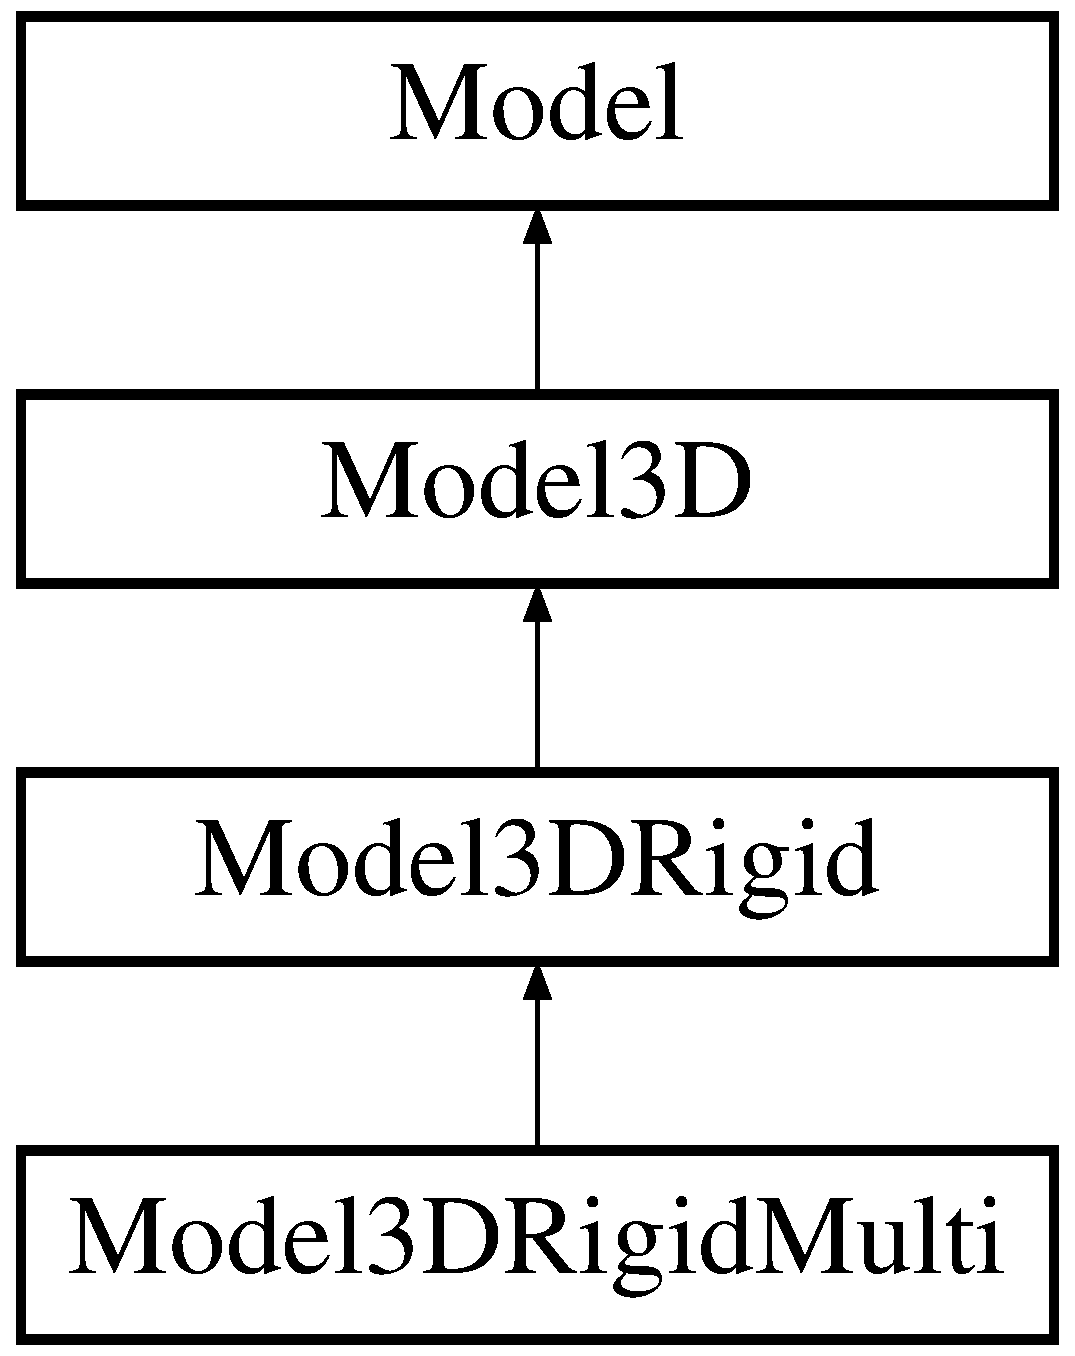
\includegraphics[height=4cm]{class_Model3DRigidMulti}
\end{center}
\end{figure}
\subsection*{Public Methods}
\begin{CompactItemize}
\item 
{\bf Model3DRigid\-Multi} (string path)
\item 
virtual {\bf $\sim$Model3DRigid\-Multi} ()
\item 
virtual double {\bf Metric} (const {\bf MSLVector} \&x1, const {\bf MSLVector} \&x2)
\begin{CompactList}\small\item\em A distance metric, which is Euclidean in the base class.\item\end{CompactList}\item 
virtual {\bf MSLVector} {\bf Linear\-Interpolate} (const {\bf MSLVector} \&x1, const {\bf MSLVector} \&x2, const double \&a)
\begin{CompactList}\small\item\em Linearly interpolate two state while respecting topology.\item\end{CompactList}\end{CompactItemize}
\subsection*{Public Attributes}
\begin{CompactItemize}
\item 
int {\bf Num\-Bodies}
\end{CompactItemize}


\subsection{Detailed Description}
A collection of free-floating bodies in a 3D world.



\subsection{Constructor \& Destructor Documentation}
\index{Model3DRigidMulti@{Model3DRigid\-Multi}!Model3DRigidMulti@{Model3DRigidMulti}}
\index{Model3DRigidMulti@{Model3DRigidMulti}!Model3DRigidMulti@{Model3DRigid\-Multi}}
\subsubsection{\setlength{\rightskip}{0pt plus 5cm}Model3DRigid\-Multi::Model3DRigid\-Multi (string {\em path})}\label{class_Model3DRigidMulti_a0}


\index{Model3DRigidMulti@{Model3DRigid\-Multi}!~Model3DRigidMulti@{$\sim$Model3DRigidMulti}}
\index{~Model3DRigidMulti@{$\sim$Model3DRigidMulti}!Model3DRigidMulti@{Model3DRigid\-Multi}}
\subsubsection{\setlength{\rightskip}{0pt plus 5cm}Model3DRigid\-Multi::$\sim$Model3DRigid\-Multi ()\hspace{0.3cm}{\tt  [inline, virtual]}}\label{class_Model3DRigidMulti_a1}




\subsection{Member Function Documentation}
\index{Model3DRigidMulti@{Model3DRigid\-Multi}!LinearInterpolate@{LinearInterpolate}}
\index{LinearInterpolate@{LinearInterpolate}!Model3DRigidMulti@{Model3DRigid\-Multi}}
\subsubsection{\setlength{\rightskip}{0pt plus 5cm}virtual {\bf MSLVector} Model3DRigid\-Multi::Linear\-Interpolate (const {\bf MSLVector} \& {\em x1}, const {\bf MSLVector} \& {\em x2}, const double \& {\em a})\hspace{0.3cm}{\tt  [virtual]}}\label{class_Model3DRigidMulti_a3}


Linearly interpolate two state while respecting topology.

If a=0, then x1 is returned; if a=1, then x2 is returned. All intermediate values of \$a $\backslash$in [0,1]\$ yield intermediate states. This method is defined by {\bf Model} {\rm (p.\,\pageref{class_Model})}. 

Reimplemented from {\bf Model3DRigid} {\rm (p.\,\pageref{class_Model3DRigid_a5})}.\index{Model3DRigidMulti@{Model3DRigid\-Multi}!Metric@{Metric}}
\index{Metric@{Metric}!Model3DRigidMulti@{Model3DRigid\-Multi}}
\subsubsection{\setlength{\rightskip}{0pt plus 5cm}virtual double Model3DRigid\-Multi::Metric (const {\bf MSLVector} \& {\em x1}, const {\bf MSLVector} \& {\em x2})\hspace{0.3cm}{\tt  [virtual]}}\label{class_Model3DRigidMulti_a2}


A distance metric, which is Euclidean in the base class.



Reimplemented from {\bf Model3DRigid} {\rm (p.\,\pageref{class_Model3DRigid_a4})}.

\subsection{Member Data Documentation}
\index{Model3DRigidMulti@{Model3DRigid\-Multi}!NumBodies@{NumBodies}}
\index{NumBodies@{NumBodies}!Model3DRigidMulti@{Model3DRigid\-Multi}}
\subsubsection{\setlength{\rightskip}{0pt plus 5cm}int Model3DRigid\-Multi::Num\-Bodies}\label{class_Model3DRigidMulti_m0}




The documentation for this class was generated from the following file:\begin{CompactItemize}
\item 
{\bf model3d.h}\end{CompactItemize}
